\section{Results Consideration}

The results of genetic algorithm are shown in tables~\ref{tab:onesideLamps} and \ref{tab:twosideLamps}. The results should be considered as solutions close to optimum specified by the fitness function. Genetic algorithms are capable of multi parametric optimization, but they are also unable to give exact solutions (\cite{Zelinka2009}, \cite{Fogel2006}). The perfect optimum must be found by some other usually deterministic method. These methods usually start from the solution found by genetic algorithms.

The algorithm found different solution during the testing, that fulfill defined constraints. This is normal behavior of the algorithm. If more than one solution exist with close maximums of the fitness, then the algorithm randomly found one of them. There can be some preferences from designer. For example he might prefer that the pillars highs cannot be more than 10~m or that the distances between the pillars must be as far as possible an so on. These preferences must be then somehow included to set limits of searched values or in the composition of the fitness function. Authors set pretty lose limits, therefore there are more than one close to optimal solution for some types of the lamps. Other possible solutions are not presented in table~\ref{tab:onesideLamps} nor in table~\ref{tab:twosideLamps}.
 
\begin{table}[htb]
	\renewcommand{\arraystretch}{1.3}
	\caption{Results for one side lamp placement}
 	\label{tab:onesideLamps}
	\centering
  \begin{tabular}{ l | c | c | c | c | c | c | c }
    \hline
    \textbf{Type} & $D_X$ & $D_Y$ & $Z$ & $\alpha$ & $\overline{E}$ & $E_{min}$ & $\overline{E}_o$\\ 
    & (m) & (m) & (m) & ($^\circ$) & (lx) & (lx) & (lx)\\ \hline
    ATOS 70W A1 & 37.5 & 0.19 & 6.77 & 0.70 & 8.07 & 1.64 & 7.58 \\ \hline
    ATOS 70W A2 & 41.8 & -0.73 & 6.54 & 2.43 & 8.13 & 1.42 & 7.25\\ \hline
    ATOS 70W A3 & 44.9 & -1.69 & 6.47 & 3.34 & 8.15 & 1.36 & 6.86\\ \hline
    ATOS 70W A4 & 47.9 & -0.41 & 6.97 & 3.59 & 8.14 & 1.36 & 6.72\\ \hline\hline
    ATOS 70W B1 & 36.8 & 0.09 & 6.86 & 2.77 & 8.13 & 1.31 & 7.70\\ \hline
    ATOS 70W B2 & 41.1 & -1.29 & 7.28 & 1.69 & 8.14 & 1.34 & 7.17\\ \hline
    ATOS 70W B3 & 45.4 & -1.40 & 7.76 & 1.29 & 8.14 & 1.55 & 6.84\\ \hline
    ATOS 70W B4 & 49.5 & -1.59 & 7.69 & 2.54 & 8.13 & 1.72 & 6.76\\ \hline\hline
    ATOS 70W C1 & 37.6 & -0.60 & 6.23 & 6.57 & 8.13 & 1.38 & 7.65\\ \hline
    ATOS 70W C2 & 41.14 & -0.59 & 6.72 & 1.86 & 8.14 & 1.50 & 7.30\\ \hline
    ATOS 70W C3 & 45.1 & -0.75 & 6.56 & 5.49 & 8.14 & 1.31 & 6.91\\ \hline
    ATOS 70W C4 & 48.0 & 0.03 & 6.85 & 6.70 & 8.14 & 1.36 & 6.92\\ \hline
  \end{tabular}
\end{table}

\begin{table}[htb]
	\renewcommand{\arraystretch}{1.3}
	\caption{Results for two sides lamp placement}
 	\label{tab:twosideLamps}
	\centering
  \begin{tabular}{ l | c | c | c | c | c | c | c }
    \hline
    \textbf{Type} & $D_X$ & $D_Y$ & $Z$ & $\alpha$ & $\overline{E}$ & $E_{min}$ & $\overline{E}_o$\\ 
    & (m) & (m) & (m) & ($^\circ$) & (lx) & (lx) & (lx)\\ \hline
    ATOS 70W A1 & 39.0 & 0.42 & 6.26 & 4.84 & 8.14 & 1.32 & 7.43 \\ \hline
    ATOS 70W A2 & 40.9 & -0.58 & 6.19 & 7.60 & 8.13 & 1.31 & 7.40\\ \hline
    ATOS 70W A3 & 44.5 & -0.90 & 6.54 & 5.40 & 8.13 & 1.35 & 6.98\\ \hline
    ATOS 70W A4 & 45.8 & -1.42 & 6.45 & 10.51 & 8.13 & 1.42 & 6.82\\ \hline\hline
    ATOS 70W B1 & 36.8 & 0.07 & 6.87 & 3.25 & 8.13 & 1.34 & 7.70\\ \hline
    ATOS 70W B2 & 41.0 & -0.46 & 7.25 & 0.81 & 8.13 & 1.35 & 7.41\\ \hline
    ATOS 70W B3 & 43.6 & -1.11 & 7.53 & 5.24 & 8.13 & 1.61 & 7.06\\ \hline
    ATOS 70W B4 & 48.51 & -1.49 & 7.34 & 8.76 & 8.13 & 1.30 & 6.73\\ \hline\hline
    ATOS 70W C1 & 37.4 & -0.45 & 6.73 & 0.55 & 8.14 & 1.60 & 7.64\\ \hline
    ATOS 70W C2 & 41.1 & -1.28 & 6.55 & 3.09 & 8.14 & 1.34 & 7.18\\ \hline
    ATOS 70W C3 & 46.0 & -0.76 & 6.95 & 1.03 & 8.13 & 1.38 & 6.68\\ \hline
    ATOS 70W C4 & 49.8 & -0.14 & 7.09 & 1.90 & 8.14 & 1.32 & 6.62\\ \hline
  \end{tabular}
\end{table}

\subsection{Example of the result}

\begin{table}[htb]
	\renewcommand{\arraystretch}{1.3}
	\caption{ATOS 70 W A1, data for graphical results in Figure}
 	\label{tab:example}
	\centering
  \begin{tabular}{ l | c | c | c | c | c | c | c }
    \hline
    \textbf{Placement} & $D_X$ & $D_Y$ & $Z$ & $\alpha$ & $\overline{E}$ & $E_{min}$ & $\overline{E}_o$\\ 
    & (m) & (m) & (m) & ($^\circ$) & (lx) & (lx) & (lx)\\ \hline
    one side & 39.8 & 0.67 & 6.22 & 3.15 & 8.14 & 1.31 & 7.40\\ \hline
    two side & 39.2 & -0.21 & 6.24 & 3.85 & 8.14 & 1.32 & 7.55 \\ \hline
  \end{tabular}
\end{table}

\begin{figure}[t]
        \centering
        \subfloat[Fitness function during the optimization]{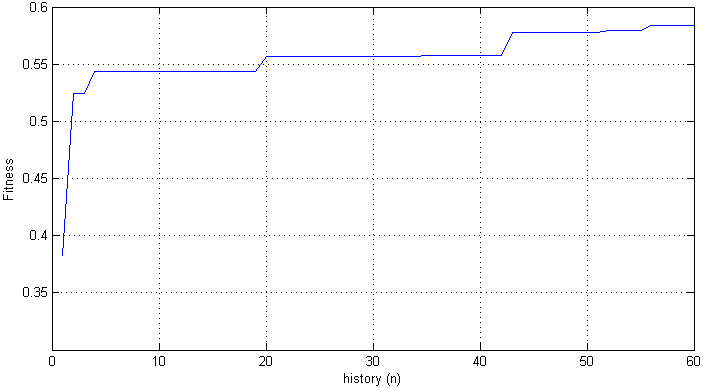
\includegraphics[width=\columnwidth]{GrafyOS_Fit}}\\
        \subfloat[Color map represents illuminance on the road, best offspring]{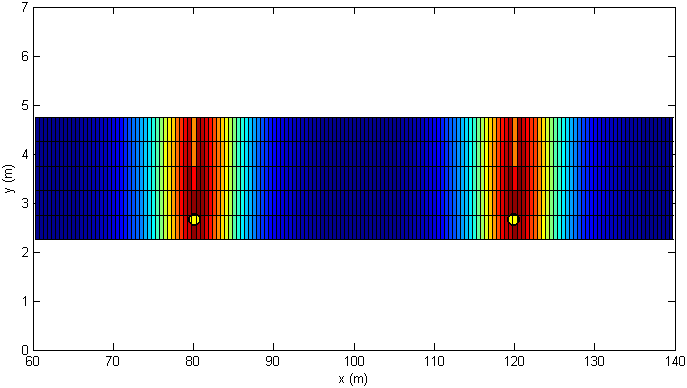
\includegraphics[width=\columnwidth]{GrafyOS_Fill}}\\
        \subfloat[Illuminance on the road, best offspring]{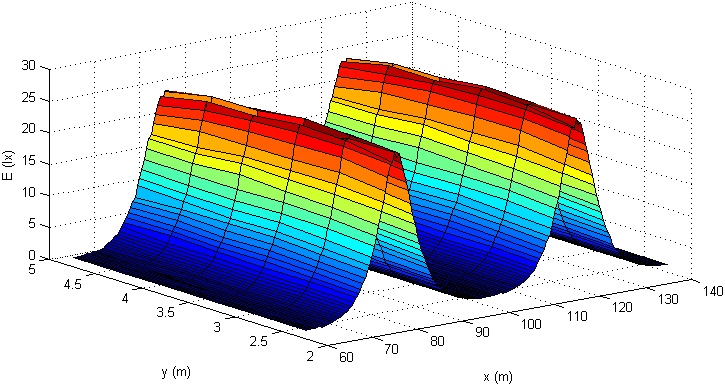
\includegraphics[width=\columnwidth]{GrafyOS_3D}}
        \label{fig:exampleOS}
        \caption{Example of result of lamp ATOS~70~W~A1 for one side placement}
\end{figure}

\begin{figure}[t]
        \centering
        \subfloat[Fitness function during the optimization]{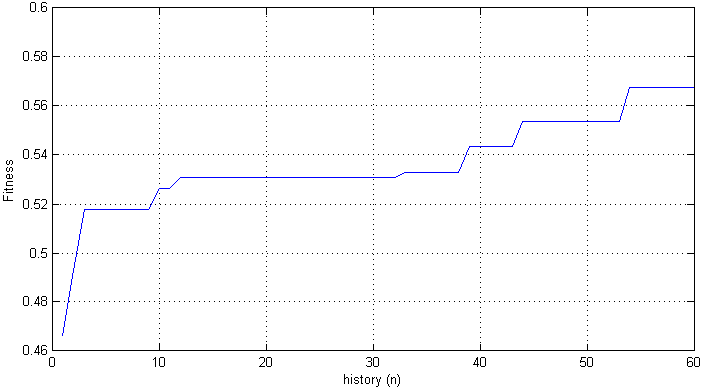
\includegraphics[width=\columnwidth]{GrafyTS_Fit}}\\
        \subfloat[Color map represents illuminance on the road, best offspring]{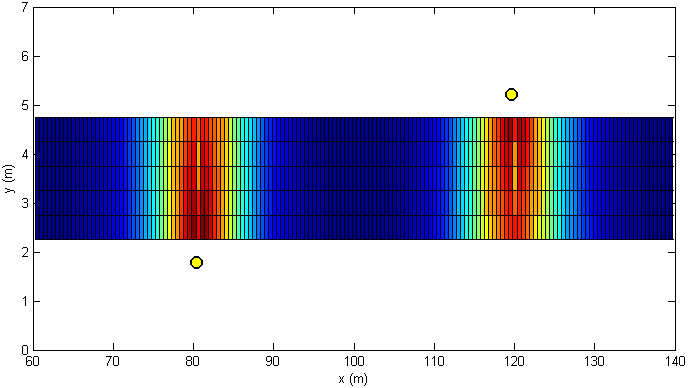
\includegraphics[width=\columnwidth]{GrafyTS_Fill}}\\
        \subfloat[Illuminance on the road, best offspring]{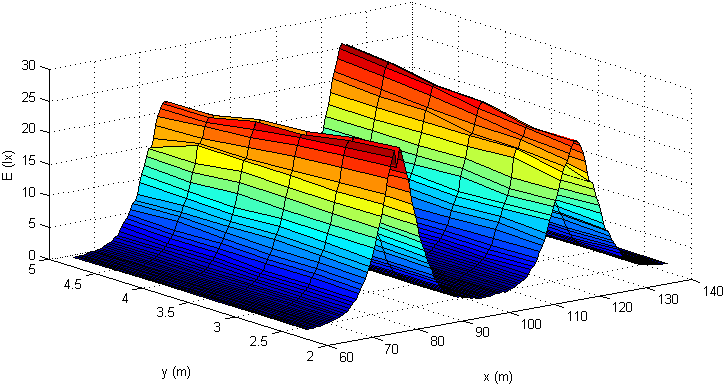
\includegraphics[width=\columnwidth]{GrafyTS_3D}}
        \label{fig:exampleTS}
        \caption{Example of result of lamp ATOS~70~W~A1 for two side placement}
\end{figure}